\section{Sistema Nervioso}

El sistema nervioso se estudia principalmente en dos partes, sistema nervioso periférico (SNP), y sistema nervioso central (SNC). SNC es donde nos enfocaremos, se compone principalmente por la medula espinal y el encéfalo. Es en el encéfalo donde se encuentra principalmente el cerebro, cerebelo, y el tallo encefálico.\cite{sistNerv}   

\textbf{¿Qué es un nervio?}

Un nervio es una estructura conductora de impulsos nerviosos.
Esta compuesto por una colección de axones los cuales son prolongaciones largas y delgadas de las células nerviosas agrupados en fibras y rodeados de vasos sanguíneos.
% Los axones, responsables de transmitir señales eléctricas y químicas entre las células nerviosas, forman una especie de "cable" a través del cual viajan los impulsos nerviosos. 
 Se origina desde la médula espinal o el encéfalo. %(31 pares de nervios raquídeos) o el encéfalo (12 pares de nervios craneales).

\textbf{¿Qué son los nervios?}

En conjunto son la escrutura organizada por tejido conectivo en el sistema nervioso, encargada de transmitir información entre diferentes partes del cuerpo del SNP y del SNC, permitiendo así el control y coordinación eficientes de las actividades corporales.
Se extienden desde el cráneo y la médula espinal para abarcar todo el cuerpo humano. \cite{princNS5}


 
 
Estos pueden ser clasificados en:

\begin{itemize}
\item \textbf{Motores} salidas, ejecución/acción, se conectan y ejercen su acción sobre los músculos.
\item \textbf{Sensitivos} reciben señales de entrada, como en ojos, oídos y piel.
\item \textbf{Mixtos} son mayoría, tienen tanto fibras sensitivas como motoras.
\end{itemize}

Las ideas tomadas del SNC para el desarrollo de las RNA, son:
\begin{itemize}
 \item La serie de entradas, del mundo exterior hacia los nervios receptores.
 \item Una o varias salidas/respuestas ante un estímulo.
 \item Conexiones entre los nervios motores, sensitivos, mixtos y el encéfalo o médula espinal. 
\end{itemize}


Reflexionando sobre lo expuesto anteriormente acerca del sistema nervioso,
este lo podemos entender como un sistema que nos da la habilidad de percibir el mundo con el que interactuamos, a través de los nervios que están en nuestra piel los cuales transmiten la información hasta nuestra médula espinal o cerebelo. Este proceso nos lleva a concebir la primera y segunda idea: un conjunto de estímulos sensoriales que incitan, una o varias respuesta de nuestro cuerpo. La tercera idea es: la forma, la escrutura que permite hacer las debidas conexiones que llevan la información requerida por y para cada celula.

La manera en la que estan hechas estas conexiones es el punto de partida para la creatividad en la forma de modelar una Red Neuronal Artificial (RNA).

\subsection{Cerebro}

Desde la parte tangible del cerebro hasta la intangible del pensamiento, está directamente relacionada con la forma que funciona nuestro pensamiento y reacciones motoras.


El cerebro, por su gran tamaño, da lugar a un mejor registro de su actividad. Los muchos registros realizados muestran que se incrementa la circulación de la sangre en el área del cerebro con mayor actividad neuronal. Se tienen identificadas regiones que se activan ante cierto estímulo. \cite{neurona_A_cerebro}


 Se detecta cuánta sangre se está bombeando en diferentes regiones del cerebro dependiendo de los estímulos que se le presentan a una persona; o si alguna persona tiene un padecimiento, se toman escaneos para ver qué regiones del cerebro están funcionando y cuáles presentan lesiones. A partir de las lesiones y de la identificación de la actividad que ya no se puede realizar de forma normal, se infiere qué región era responsable de esa actividad que ahora está dañada.\cite{estudiosF}

Para obtener más detalle de los estudios de la actividad del cerebro, ver el documental "The Brain with David Eagleman".

\subsection{Zonas funcionales}

En el cerebro, las diversas zonas identificadas con funciones específicas, están conectadas, por una ruta que se conoce como 
 ''la ruta desde la sensación hasta la cognición'' notemos un diagrama de la parte funcional del cerebro. \cite{sensAcogn}  


 \begin{figure}[h]
  \centering
  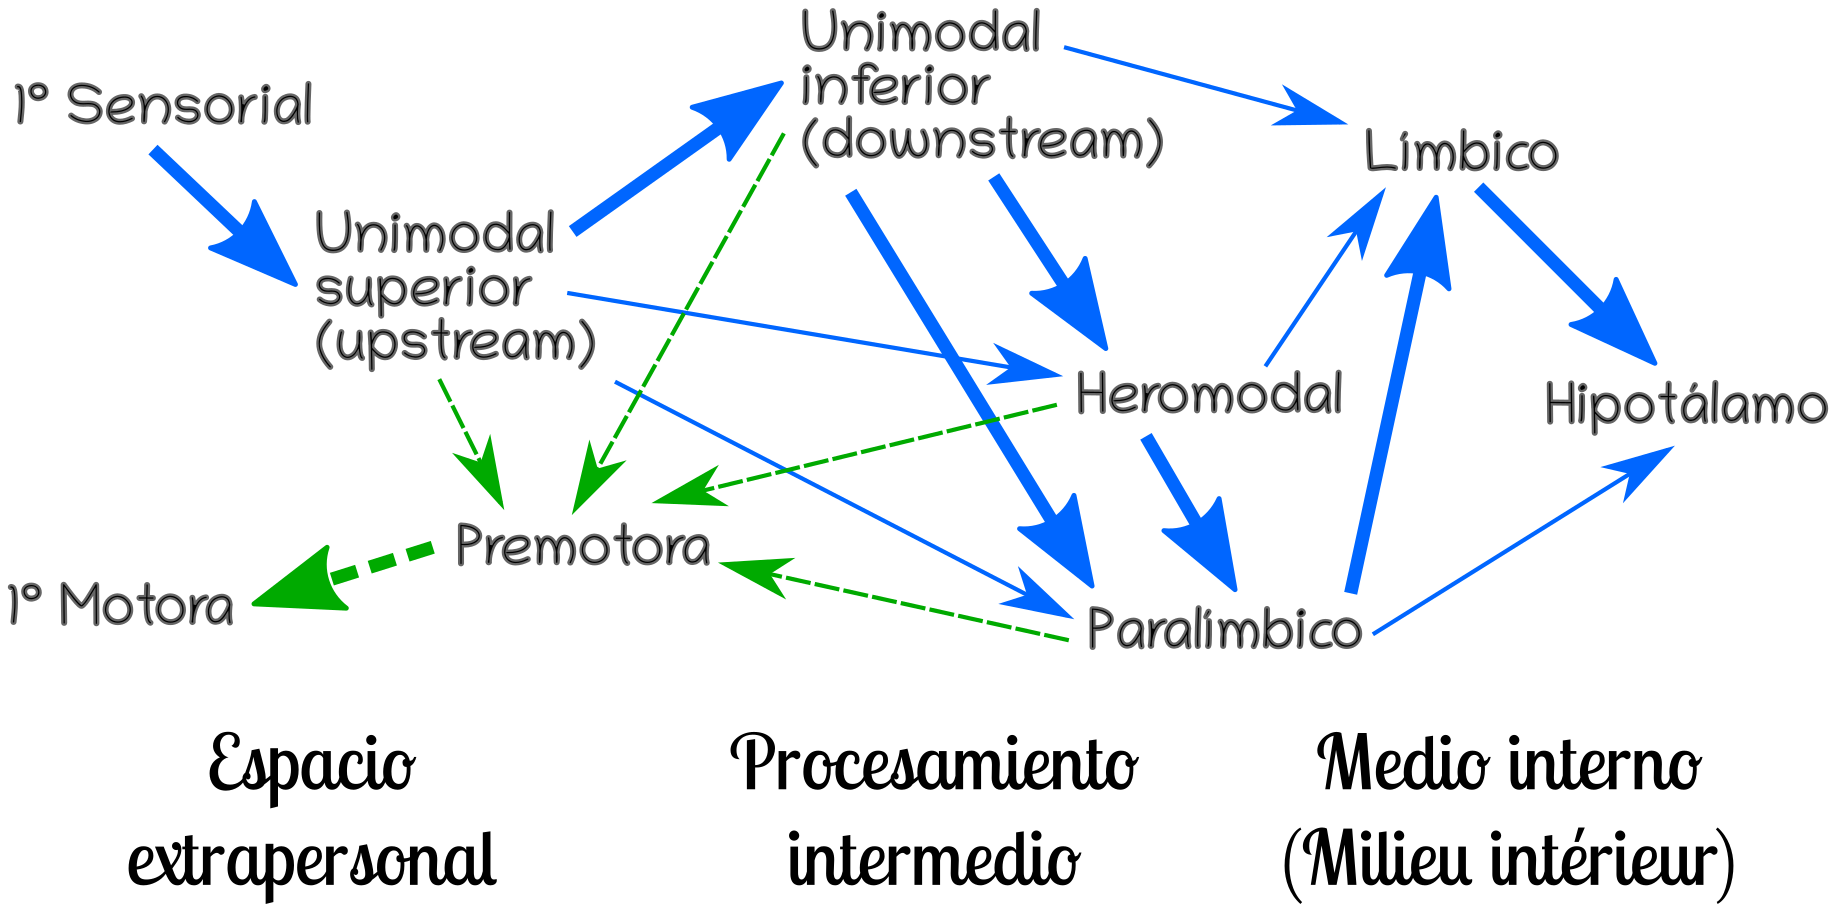
\includegraphics[width=0.9\textwidth]{../Figuras/zonasFuncionales.png}
  \caption{Diagrama de la arquitectura del cerebro a nivel funcional. Enfocado en sentido de la visión o la audición. \parencite{Mesulam1998}. Redibujado por E. Verónica Arriola Ríos}
  \label{fig:zonasFun}
 \end{figure}

Explicación: El punto de partida de la ruta es la etapa/capa sensorial, que la vamos a conciderar como \textbf{la entrada}. El cerebro está recibiendo señales/información en el momento que existe una sensación que viene del mundo exterior.

Su primera conexión es hacia la capa unimodal superior, que la vamos a conciderar como \textbf{la primera capa}. Donde se procesa la información más básica de la señal (del sentido), tales como el color, las formas o los tonos de sonido.

Luego están las capas intermedias (unimodal, heromodal, paralimbico, limbico), donde se dará un procesamiento intermedio; se juntarán varias características interpretadas por la primera capa. Conforme avance la señal a las siguientes capas, las neuronas notaran características más complejas. 

%En la capa unimodal y heteromodal se espera que la información codificada sea la persepción y una planeación motora. Es decir, que se va a formar el plan de reacción motora ante la señal. 

% En las capas paralimbicas se espera que la información codificada sea el cambio de emoción y motivación. Es decir, que no habra una reacción hacia el mundo solo hacia el cerebro y este refuerzo de señales hará un refuerzo/cambio de conducta a largo plazo.

% En las capas limbicas se espera que se codifique la regulación de la emocion, la motivación y memoria.

% Una vez llege la señal (con la codificación de todas capas por las que paso) al hipotálamo, este se encarga de coordinar las respuestas codificadas. Ya sea hacia la capa premotora o paralibica. En el caso del diagrama las flechas en color verde indican que hubo una respuesta hacia la capa premotora, que tendrá una salida hacia los nervios motores, es decir una reacción motora inmediata de la señal. 


Finalmente, llegamos al hipotálamo, que con todas las características dadas mandará a través de las capas intermedias una o varias respuestas, cuya etapa final se dará en la capa premotora, donde las neuronas de esta capa se comunican directamente con la \textbf{salida} motora.







